\setcounter{ExampleCounter}{1}
Suppose you had the following histogram of a frequency distribution:
\begin{center}
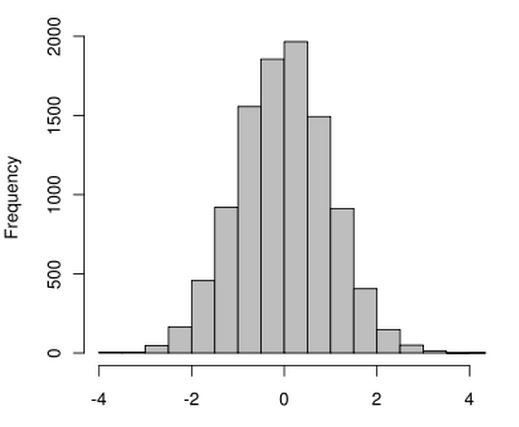
\includegraphics[height=2.0in]{NormHistgrm_Kierano}
\end{center}
If we connected the bars via a smooth line, we would get something like this:
\begin{center}
\begin{tikzpicture}
\begin{axis}[
  no markers, domain=-4:4, samples=100,
  axis lines*=none,
  hide y axis,
  every axis y label/.style={at=(current axis.above origin),anchor=south},
  every axis x label/.style={at=(current axis.right of origin),anchor=west},
  height=5cm, width=12cm,
  xtick=\empty, ytick=\empty,
  enlargelimits=false, clip=false, %axis on top,
  %grid = major
  ]
  \addplot [very thick,cyan!50!black] {gauss(0,1)};
\end{axis}

\end{tikzpicture}
\end{center}
This is known as a \textbf{bell-shaped curve}. It is the most widely used and abused graph in many disciplines, from psychology, business and economics to science and medicine. This curve is also known as a ``Gaussian Curve,'' named after Carl Friedrich Gauss, the famous mathematician. The bell-shaped curve is the graph of the \textbf{normal distribution}, the most important of all distributions in statistics. 

\marginnote{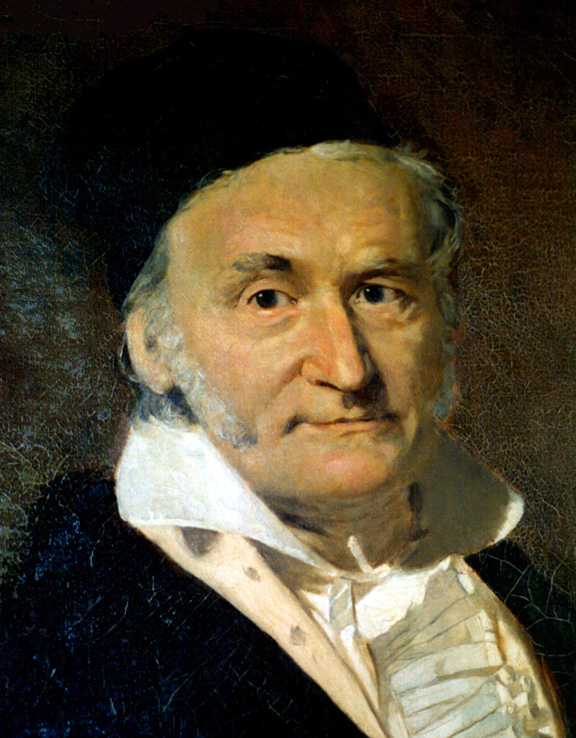
\includegraphics[height=1.0in]{Gauss}}
\marginnote{C.F.Gauss}[3 cm]

Notice how the bell-shaped curve is symmetric about a central line. The center of the curve is the mean. But it's also the median and the mode. Hence, for all bell-shaped curves, the mean is equal to the median which is equal to the mode. 

What kind of data does the bell-shaped curve describe? Data that has many middle or average values and fewer high or low values. Think of men's heights. There are many men of average height, yet few very tall and few very short men. The same applies to women's heights. Hence, height is a variable that is \textbf{normally distributed}. 

IQ is also normally distributed. Most people have average IQs. There are very few people with extremely high IQs and very few with extremely low IQs. 

There are many variables that are normally distributed. Any variable that has a bell-shaped distribution is said to be normally distributed. Different variables have different bell-shaped curves. 
\begin{center}
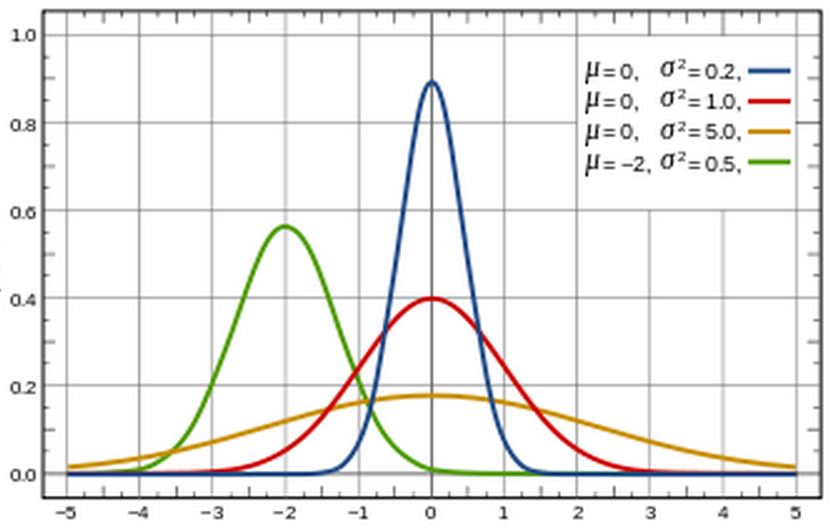
\includegraphics[height=2.5in]{MultNorm}
\end{center}
How the curve looks depends on the mean and standard deviation. Changing the mean shifts the curve right and left. Changing the standard deviation changes the shape of the curve: a large standard deviation results in a wide curve and a small standard deviation results in a narrow curve. 

The blue curve in the above diagram has a mean of 0, whereas the green curve has a mean of $-2$. Since the green curve's mean is lower, it is to the left of the blue curve (think about where the numbers are on the number line).

The standard deviation of the blue curve is 0.45. The standard deviation of the green curve is 0.71. Since the standard deviation of the green curve is larger, it is wider compared to the blue curve.

On the same diagram, notice the red curve. It has a mean of 0 and a standard deviation of 1. This is a special curve known as the \textbf{standard normal curve}.

\subsection{Z-Scores}
The normal distribution is precisely defined enough that if we have some information about a particular normally distributed quantity--specifically its mean and standard deviation--we can tell precisely where a specific data point falls in that distribution.  In other words, we can answer questions like: is it unusual for a man to be over 6'4''?  Just \textit{how} unusual?

We can describe the position of a data point in a normal distribution using its \textbf{z-score}, which measures by how many standard deviations a data point differs from the mean.

For instance, suppose a particular data set is normally distributed with a mean of 100 and a standard deviation of 10.  Then a data point of 110 has a $z$-score of 1, a data point of 150 has a $z$-score of 5, and a data point of 70 has a $z$-score of $-3$ (negative because it is \textit{below} the mean).

To find the $z$-score for a data point in a data set with a known mean and standard deviation, we just need to find its distance from the mean, and then divide that by the standard deviation to find out how many steps it will take from the mean to reach it.

\begin{formula}{Z-Scores}
If $x$ is a data value in a data set with mean $\overline{x}$ and standard deviation $s$, the $z$-score that corresponds to that data value is
\begin{align*}
z\textrm{-score } &= \dfrac{\textrm{data value } - \textrm{ mean}}{\textrm{standard deviation}}\\
z &= \dfrac{x-\overline{x}}{s}
\end{align*}
\end{formula}

\begin{example}[https://www.youtube.com/watch?v=DKmhYrgywMc]{Female Heights}
Female adult height is normally distributed with a mean of 65 in. and a standard deviation of 3.5 in.\\

Find the $z$-scores of the following heights:
\begin{enumerate}[(a)]
\item 58 in.
\item 71 in.
\end{enumerate}

\marginnote{\bfseries Solution}
\begin{enumerate}[(a)]
\item The $z$-score corresponding to 58 in. is
\[z=\dfrac{58-65}{3.5} = -2\]
\item The $z$-score corresponding to 71 in. is
\[z = \dfrac{71-65}{3.5} = 1.71\]
\end{enumerate}
Thus, a woman at 71 in. tall is 1.71 standard deviations above the mean, while a woman at 58 in. is 2 standard deviations below the mean.
\end{example}

\begin{try}[http://www.izzomath.com/103text/stats/example4.1/story.html]
Scores on the SAT and ACT are normally distributed:
\begin{center}
\begin{tabular}{l l l}
Test & Mean & Std. Deviation\\
\hline
SAT & 500 & 100\\
ACT & 18 & 6
\end{tabular}
\end{center}
You score 550 on the SAT and 24 on the ACT.  On which test did you have a better score, relative to everyone else who took the test?
\end{try}

\begin{example}[https://www.youtube.com/watch?v=qfg_DWgY3Hg]{Working Backward from Z-Scores}
Scores on an IQ test are normally distributed with a mean of 100 and a standard deviation of 15.  Find the IQ score that corresponds to each of the following $z$-scores.
\begin{enumerate}[(a)]
\item $-1.5$
\item $2.05$
\end{enumerate}

\marginnote{\bfseries Solution}
Recall that $z=\dfrac{\textrm{data value } - \textrm{ mean}}{\textrm{standard deviation}}$
\begin{enumerate}[(a)]
\item If the $z$-score is $-1.5$:
\[-1.5=\dfrac{\textrm{IQ } - 100}{15} \longrightarrow -22.5 = \textrm{IQ } - 100 \longrightarrow \textrm{IQ } = 77.5\]
\item If the $z$-score is $2.05$:
\[2.05=\dfrac{\textrm{IQ } - 100}{15} \longrightarrow 30.75 = \textrm{IQ } - 100 \longrightarrow \textrm{IQ } = 130.75\]
\end{enumerate}
\end{example}

\subsection{The Empirical Rule}

Not only do the mean and standard deviation define the normal distribution, they play a vital part in the Empirical Rule. This important rule allows us to determine whether a particular data point is unusual or not by comparing it to where most of the data falls.  The Empirical Rule gives a precise prediction about where the data is distributed.

\begin{proc}{The Empirical Rule}

Approximately 68\% of the data is within \textbf{one} standard deviation of the mean.
Approximately 95\% of the data is within \textbf{two} standard deviations of the mean. 
Approximately 99.7\% of the data is within \textbf{three} standard deviations of the mean.


\begin{center}
\begin{tikzpicture}
\begin{axis}[
  no markers, domain=-4:4, samples=100,
  axis lines*=none, xlabel=$x$,
  hide y axis,
  every axis y label/.style={at=(current axis.above origin),anchor=south},
  every axis x label/.style={at=(current axis.right of origin),anchor=west},
  height=5cm, width=12cm,
  xtick={-3,-2,-1,0,1,2,3}, ytick=\empty,
  xticklabels={$\mu-3\sigma$,$\mu-2\sigma$,$\mu-\sigma$,$\mu$,$\mu+\sigma$,$\mu+2\sigma$,$\mu+3\sigma$},
  enlargelimits=false, clip=false, %axis on top,
  grid = major
  ]
  \addplot [fill=cyan!20, draw=none, domain=-1:1] {gauss(0,1)} \closedcycle;
  \addplot [fill=yellow!20, draw=none, domain=-2:-1] {gauss(0,1)} \closedcycle;
  \addplot [fill=yellow!20, draw=none, domain=1:2] {gauss(0,1)} \closedcycle;
  \addplot [fill=green!20, draw=none, domain=-3:-2] {gauss(0,1)} \closedcycle;
  \addplot [fill=green!20, draw=none, domain=2:3] {gauss(0,1)} \closedcycle;
  \addplot [very thick,cyan!50!black] {gauss(0,1)};


\draw [yshift=2.5cm, latex-latex](axis cs:-1,0) -- node [fill=white] {68\%} (axis cs:1,0);
\draw [yshift=1.5cm, latex-latex](axis cs:-2,0) -- node [fill=white] {95\%} (axis cs:2,0);
\draw [yshift=0.5cm, latex-latex](axis cs:-3,0) -- node [fill=white] {99.7\%} (axis cs:3,0);
\end{axis}

\end{tikzpicture}
\end{center}

Note that this diagram uses $\mu$ for the population mean (as opposed to $\overline{x}$ for the sample mean) and $\sigma$ for the population standard deviation (as opposed to $s$ for the sample standard deviation).
\end{proc}

As you can see, another name for the Empirical Rule is the "68-95-99.7 Rule."  Let's use this rule to look at IQ in the population.
\vfill
\pagebreak

\begin{example}[https://www.youtube.com/watch?v=cTRr0B5Cp8k]{The Intelligence Quotient}
IQ is normally distributed with a mean of 100 and a standard deviation of 15. Use the Empirical Rule to the find the data that is within one, two, and three standard deviations of the mean.

\marginnote{\bfseries Solution}
\begin{enumerate}
\item{68\% of the data is within one standard deviation of the mean.
\\ 
 IQ = mean $\pm (1 \cdot$ standard deviation $) = 100 \pm (1 \cdot 15) = 100 \pm 15 = (85, 115)$
 Thus, 68\% of people have an IQ between 85 and 115.
}
\item{95\% of the data is within two standard deviations of the mean.
\\ 
 IQ = mean $\pm (2 \cdot$ standard deviation $) = 100 \pm (2 \cdot 15) = 100 \pm 30 = (70, 130)$
 Thus, 95\% of people have an IQ between 70 and 130.
}
\item{99.7\% of the data is within three standard deviations of the mean.
\\ 
 IQ = mean $\pm (3 \cdot$ standard deviation $) = 100 \pm (3 \cdot 15) = 100 \pm 45 = (55, 145)$
Thus, 99.7\% of people have an IQ between 55 and 145.
}
\end{enumerate}
\begin{center}
\begin{tikzpicture}
\begin{axis}[
  no markers, domain=-4:4, samples=100,
  axis lines*=none, xlabel=$x$,
  hide y axis,
  every axis y label/.style={at=(current axis.above origin),anchor=south},
  every axis x label/.style={at=(current axis.right of origin),anchor=west},
  height=5cm, width=12cm,
  xtick={-3,-2,-1,0,1,2,3}, ytick=\empty,
  xticklabels={55,70,85,100,115,130,145},
  enlargelimits=false, clip=false, %axis on top,
  grid = major
  ]
  \addplot [fill=cyan!20, draw=none, domain=-1:1] {gauss(0,1)} \closedcycle;
  \addplot [fill=yellow!20, draw=none, domain=-2:-1] {gauss(0,1)} \closedcycle;
  \addplot [fill=yellow!20, draw=none, domain=1:2] {gauss(0,1)} \closedcycle;
  \addplot [fill=green!20, draw=none, domain=-3:-2] {gauss(0,1)} \closedcycle;
  \addplot [fill=green!20, draw=none, domain=2:3] {gauss(0,1)} \closedcycle;
  \addplot [very thick,cyan!50!black] {gauss(0,1)};


\draw [yshift=2.5cm, latex-latex](axis cs:-1,0) -- node [fill=white] {68\%} (axis cs:1,0);
\draw [yshift=1.5cm, latex-latex](axis cs:-2,0) -- node [fill=white] {95\%} (axis cs:2,0);
\draw [yshift=0.5cm, latex-latex](axis cs:-3,0) -- node [fill=white] {99.7\%} (axis cs:3,0);
\end{axis}

\end{tikzpicture}
\end{center}

Again, this rule gives a way to decide whether a data point is unusual or not.  An IQ of over 130 is very unusual, and an IQ of over 145 is even more so.\\

Since 99.7\% have IQs in the range from 55 to 145, only 0.3\% of people have IQs outside that range.  Since the bell curve is symmetric, half of those, or 0.15\% of people (15 people out of 1000) have IQs over 145.
\end{example}

\begin{try}[http://www.izzomath.com/103text/stats/example4.3/story.html]
The mean height of boys 15 to 18-years old from Chile is 170 cm with a standard deviation of 6 cm. Male heights are known to be normally distributed. Using the Empirical Rule, find the range of heights that contain approximately 68\%, 95\%, and 99.7\% of the data.
\end{try}

\begin{example}[https://www.youtube.com/watch?v=XcZCDQln9L0]{College Entrance Exams}
The scores on a college entrance exam are normally distributed with a mean of 52 points and a standard deviation of 11 points. About 95\% of the values lie between what two scores?\\

\marginnote{\bfseries Solution}
We know 95\% of the data is within two standard deviations of the mean. 

Scores = Mean $\pm$ 2$\cdot$ Standard Deviation $= 52 \pm 2\cdot11 = 52 \pm 22 = (30, 74)$.

Hence, 95\% of the values fall between a score of 30 and a score of 74.
\end{example}
\pagebreak

Let's go back to the figure from the first example:
\begin{center}
\begin{tikzpicture}
\begin{axis}[
  no markers, domain=-4:4, samples=100,
  axis lines*=none, xlabel=$x$,
  hide y axis,
  every axis y label/.style={at=(current axis.above origin),anchor=south},
  every axis x label/.style={at=(current axis.right of origin),anchor=west},
  height=5cm, width=12cm,
  xtick={-3,-2,-1,0,1,2,3}, ytick=\empty,
  xticklabels={55,70,85,100,115,130,145},
  enlargelimits=false, clip=false, %axis on top,
  grid = major
  ]
  \addplot [fill=cyan!20, draw=none, domain=-1:1] {gauss(0,1)} \closedcycle;
  \addplot [fill=yellow!20, draw=none, domain=-2:-1] {gauss(0,1)} \closedcycle;
  \addplot [fill=yellow!20, draw=none, domain=1:2] {gauss(0,1)} \closedcycle;
  \addplot [fill=green!20, draw=none, domain=-3:-2] {gauss(0,1)} \closedcycle;
  \addplot [fill=green!20, draw=none, domain=2:3] {gauss(0,1)} \closedcycle;
  \addplot [very thick,cyan!50!black] {gauss(0,1)};


\draw [yshift=2.5cm, latex-latex](axis cs:-1,0) -- node [fill=white] {68\%} (axis cs:1,0);
\draw [yshift=1.5cm, latex-latex](axis cs:-2,0) -- node [fill=white] {95\%} (axis cs:2,0);
\draw [yshift=0.5cm, latex-latex](axis cs:-3,0) -- node [fill=white] {99.7\%} (axis cs:3,0);
\end{axis}

\end{tikzpicture}
\end{center}

What if we want to find what percentage of the data falls in some other range?  Like what about the percentage of IQs that fall between 100 and 115?  Or above 85?  Between 70 and 115?

All of this can be done with a little clever analysis of the figure above.  We just need to divide it up into segments that are each one standard deviation (15 IQ points) wide and figure out what percentage of the data is in each slice.

First of all, notice that the center region (between 85 and 115) contains 68\% of the data.  Because the graph is symmetric, we can conclude that each half of that contains 34\%.

Next, the two yellow regions together contain $95\%-68\% = 27\%$, so each region contains half of that, or 13.5\%.  Similarly, the two green regions account for $99.7\%-95\% = 4.7\%$, so each of them contains 2.35\% of the data.  Finally, the tails outside the green account for the remaining 0.3\% of the data, so each side contains 0.15\%.

\begin{center}
\begin{tikzpicture}
\begin{axis}[
  no markers, domain=-4:4, samples=100,
  axis lines*=none, xlabel=$x$,
  hide y axis,
  every axis y label/.style={at=(current axis.above origin),anchor=south},
  every axis x label/.style={at=(current axis.right of origin),anchor=west},
  height=5cm, width=12cm,
  xtick={-3,-2,-1,0,1,2,3}, ytick=\empty,
  xticklabels={55,70,85,100,115,130,145},
  enlargelimits=false, clip=false, axis on top,
  grid = major
  ]
  \addplot [fill=cyan!20, draw=none, domain=-1:1] {gauss(0,1)} \closedcycle;
  \addplot [fill=yellow!20, draw=none, domain=-2:-1] {gauss(0,1)} \closedcycle;
  \addplot [fill=yellow!20, draw=none, domain=1:2] {gauss(0,1)} \closedcycle;
  \addplot [fill=green!20, draw=none, domain=-3:-2] {gauss(0,1)} \closedcycle;
  \addplot [fill=green!20, draw=none, domain=2:3] {gauss(0,1)} \closedcycle;
  \addplot [very thick,cyan!50!black] {gauss(0,1)};

\draw [yshift=2cm,xshift=5.9cm] node {34\%};
\draw [yshift=2cm,xshift=4.6cm] node {34\%};
\draw [yshift=0.5cm,xshift=7.2cm] node {13.5\%};
\draw [yshift=0.5cm,xshift=3.3cm] node {13.5\%};
\draw [yshift=1cm,xshift=8.5cm] node {2.35\%};
\draw [yshift=1cm,xshift=2cm] node {2.35\%};
\draw [yshift=1cm,xshift=9.8cm] node {0.15\%};
\draw [yshift=1cm,xshift=0.7cm] node {0.15\%};
\draw [yshift=4cm, latex-latex](axis cs:-1,0) -- node [fill=white] {68\%} (axis cs:1,0);
\draw [yshift=5cm, latex-latex](axis cs:-2,0) -- node [fill=white] {95\%} (axis cs:2,0);
\draw [yshift=6cm, latex-latex](axis cs:-3,0) -- node [fill=white] {99.7\%} (axis cs:3,0);
\end{axis}

\end{tikzpicture}
\end{center}

The important point is not to memorize these percentages, but rather to understand how we figured them out.  If you can follow and recreate that process, all you'll have to memorize is the 68--95--99.7 part, and you can reproduce a picture like that one in a minute or two of quick thought.  Once you can do that, you can answer questions like the following one.
\vfill
\pagebreak

\begin{example}[https://www.youtube.com/watch?v=E8rczzYhOL4]{Car Sales}
Suppose you know that the prices paid for cars are normally distributed with a mean of \$17,000 and a standard deviation of \$500.  Use the 68--95--99.7 Rule to find the percentage of buyers who paid
\begin{center}
\begin{tabular}{l l}
(a) between \$16,500 and \$17,500 & (b) between \$17,500 and \$18,000\\
(c) between \$16,000 and \$17,000 & (d) between \$16,500 and \$18,000\\
(e) below \$16,000 & (f) above \$18,500
\end{tabular}
\end{center}

\marginnote{\bfseries Solution}
We can use the same process that was just described to build the following diagram, using the given mean and standard deviation.
\begin{center}
\begin{tikzpicture}
\begin{axis}[
  no markers, domain=-4:4, samples=100,
  axis lines*=none, xlabel=$x$,
  hide y axis,
  every axis y label/.style={at=(current axis.above origin),anchor=south},
  every axis x label/.style={at=(current axis.right of origin),anchor=west},
  height=5cm, width=12cm,
  xtick={-3,-2,-1,0,1,2,3}, ytick=\empty,
  xticklabels={{\$15,500},{\$16,000},{\$16,500},{\$17,000},{\$17,500},{\$18,000},{\$18,500}},
  enlargelimits=false, clip=false, axis on top,
  grid = major
  ]
  \addplot [fill=cyan!20, draw=none, domain=-1:1] {gauss(0,1)} \closedcycle;
  \addplot [fill=yellow!20, draw=none, domain=-2:-1] {gauss(0,1)} \closedcycle;
  \addplot [fill=yellow!20, draw=none, domain=1:2] {gauss(0,1)} \closedcycle;
  \addplot [fill=green!20, draw=none, domain=-3:-2] {gauss(0,1)} \closedcycle;
  \addplot [fill=green!20, draw=none, domain=2:3] {gauss(0,1)} \closedcycle;
  \addplot [very thick,cyan!50!black] {gauss(0,1)};

\draw [yshift=2cm,xshift=5.9cm] node {34\%};
\draw [yshift=2cm,xshift=4.6cm] node {34\%};
\draw [yshift=0.5cm,xshift=7.2cm] node {13.5\%};
\draw [yshift=0.5cm,xshift=3.3cm] node {13.5\%};
\draw [yshift=1cm,xshift=8.5cm] node {2.35\%};
\draw [yshift=1cm,xshift=2cm] node {2.35\%};
\draw [yshift=1cm,xshift=9.8cm] node {0.15\%};
\draw [yshift=1cm,xshift=0.7cm] node {0.15\%};
\draw [yshift=4cm, latex-latex](axis cs:-1,0) -- node [fill=white] {68\%} (axis cs:1,0);
\draw [yshift=5cm, latex-latex](axis cs:-2,0) -- node [fill=white] {95\%} (axis cs:2,0);
\draw [yshift=6cm, latex-latex](axis cs:-3,0) -- node [fill=white] {99.7\%} (axis cs:3,0);
\end{axis}

\end{tikzpicture}
\end{center}

You should be able to use the figure above to reason out that
\begin{enumerate}[(a)]
\item the percentage of buyers who spent between \$16,500 and \$17,500 was 68\%.
\item the percentage of buyers who spent between \$17,500 and \$18,000 was 13.5\%.
\item the percentage of buyers who spent between \$16,000 and \$17,000 was 47.5\%.
\item the percentage of buyers who spent between \$16,500 and \$18,000 was 81.5\%.
\item the percentage of buyers who spent below \$16,000 was 2.5\%.
\item the percentage of buyers who spent above \$18,500 was 0.15\%.
\end{enumerate}
\end{example}

\begin{try}[http://www.izzomath.com/103text/stats/example4.5/story.html]
The mean height of boys 15 to 18-years old from Chile is 170 cm with a standard deviation of 6 cm. Male heights are known to be normally distributed. Using the Empirical Rule, find
\begin{enumerate}[(a)]
\item the percentage of boys with heights between 158 and 176. 
\item the percentage of boys with heights above 188.
\item the percentage of boys with heights below 164.
\end{enumerate}
\end{try}

\subsection{The Normal Distribution and Polls}
Suppose you're tasked with conducting a straw poll to predict the victor in a close Senate race between Jonas Hawkins and Violeta Gass.  You poll (randomly, because you're a good statistics student) 500 people and ask them who they plan to vote for, and 52\% of them respond Hawkins and 48\% Gass.  Good so far, but you begin to wonder: is this really an accurate representation of the population?  You picked a good sample, but is there any way to put a number on how certain you are that your results are a valid predictor of what the population will do?

The answer is based on the Normal Distribution.  The idea is this: if we took another sample and polled them, and then another sample, and another and another, and repeated this process many times over, the results of our poll would begin to look like a normal distribution.
\begin{center}
\begin{tikzpicture}
\begin{axis}[
  no markers, domain=-4:4, samples=100,
  axis lines*=none,
  hide y axis,
  every axis y label/.style={at=(current axis.above origin),anchor=south},
  every axis x label/.style={at=(current axis.right of origin),anchor=west},
  height=3.5cm, width=8cm,
  xtick=\empty, ytick=\empty,
  enlargelimits=false, clip=false, %axis on top,
  %grid = major
  ]
  \addplot [very thick,cyan!50!black] {gauss(0,1)};
\end{axis}

\end{tikzpicture}
\end{center}

In other words, most of those polls we conducted would look similar to each other, and they would be grouped together.  There would be a few polls that would have drastically lower percentages for Hawkins, and a few would have drastically higher percentages--simply due to the inherent variability of a sample that we can never fully eliminate--but most of them would be clustered around the true percentage of the population that plan to vote for Hawkins.  In other words, the wrong polls would be rare, and the polls that are more right would be more common.

In fact, it turns out that we can specifically define this distribution as a normal distribution, which tells us that we're--for instance--95\% confident that the results we got when we took the first poll were within two standard deviations of the mean.  Now then, if we make our sample larger, it turns out that the standard deviation on this normal distribution gets smaller, so the results are more precise.

\begin{center}
\begin{tikzpicture}
\begin{axis}[
  no markers, domain=-4:4, samples=100,
  axis lines*=none,
  hide y axis,
  every axis y label/.style={at=(current axis.above origin),anchor=south},
  every axis x label/.style={at=(current axis.right of origin),anchor=west},
  height=5cm, width=12cm,
  xtick=\empty, ytick=\empty,
  enlargelimits=false, clip=false, %axis on top,
  %grid = major
  ]
  \draw [yshift=0.5cm,xshift=1.5cm] node {smaller sample};
  \draw [yshift=2.5cm,xshift=7cm] node {larger sample};
  \addplot [very thick,cyan!50!black] {gauss(0,1)};
  \addplot [very thick,cyan!50!black] {gauss(0,0.5)};
\end{axis}

\end{tikzpicture}
\end{center}

\paragraph{Margin of Error} This allows us to define something called the margin of error.  You may have seen or heard this term in the context of polls, especially political polls.  The margin of error is an inevitable part of using a sample to predict what a larger population will do, and it only depends on $n$, the size of the sample (strangely enough, it doesn't depend on the size of the population).  The larger the sample size, the smaller the margin of error will be, and thus the more precise the results of the poll will be.

\begin{formula}{Margin of Error}
If the sample size of a poll is $n$, there is at least a 95\% chance that the sample percentage lies within \[\dfrac{1}{\sqrt{n}} \times 100\%\] of the population percent.  The margin of error with a 95\% \textit{confidence level} is $\pm \dfrac{1}{\sqrt{n}} \times 100\%$.
\end{formula}

Beware, though, that you don't take for granted that the margin of error is the only thing to worry about; we've already seen that there are other sources of error, like poor sampling.  Also, we didn't even talk about other sources of bias, like self-interest or word choice.

\begin{example}[https://www.youtube.com/watch?v=V3EBPVeTaFo]{Margin of Error}
What is the margin of error on a poll with a sample size of 1000 people?\\

\marginnote{\bfseries Solution}
The margin of error is 
\[\pm \dfrac{1}{\sqrt{1000}} \times 100\% = \pm 3.16\%\]
A margin of error of about 3\% (which is common for many political polls) corresponds to a sample size of 1000.
\end{example}


\begin{exercises}
\ptwo{The widths of platinum samples manufactured at a factory are normally distributed, with a mean of 1.1 cm and a standard deviation of 0.2 cm.  Find the $z$-scores that correspond to each of the following widths.
\begin{enumerate}[(a)]
\item 1.5 cm
\item 0.94 cm
\end{enumerate}}
\ptwo{The average resting heart rate of a population is 88 beats per minute, with a standard deviation of 12 bpm.  Find the $z$-scores that correspond to each of the following heart rates.
\begin{enumerate}[(a)]
\item 120 bpm
\item 71 bpm
\end{enumerate}}

\ptwo{The average height of American adult males is 177 cm, with a standard deviation of 7.4 cm.  Meanwhile, the average height of Indian males is 165 cm, with a standard deviation of 6.7 cm.  Which is taller relative to his nationality, a 175-cm American man or a 162-cm Indian man?}
\ptwo{Kyle and Ryan take entrance exams at two different universities.  Kyle scores a 430 on an exam with a mean of 385 and a standard deviation of 70, while Ryan scores a 31 on an exam with a mean of 28 and a standard deviation of 4.5.  Which do you think is more likely to be accepted at their university of choice?}

\ptwo{A doctor measured serum HDL levels in her patients, and found that they were normally distributed with a mean of 63.4 and a standard deviation of 3.8.  Find the serum HDL levels that correspond to the following $z$-scores.
\begin{enumerate}[(a)]
\item $z=-0.85$
\item $z=1.33$
\end{enumerate}}
\ptwo{If the distribution of weight of newborn babies in Maryland is approximately normal, with a mean of 3.23 kilograms and a standard deviation of 0.87 kilograms, find the weights that correspond to the following $z$-scores.
\begin{enumerate}[(a)]
\item $z=2.20$
\item $z=-1.73$
\end{enumerate}}

\ptwo{Once again, the heights of American adult males are normally distributed with a mean of 177 cm and a standard deviation of 7.4 cm.  Find the range of heights that contain approximately
\begin{enumerate}[(a)]
\item 68\% of the data
\item 95\% of the data
\item 99.7\% of the data
\end{enumerate}}
\ptwo{Suppose again that babies' weights are normally distributed with a mean of 3.23 kg and a standard deviation of 0.87 kg.  Find the range of weights that contain approximately
\begin{enumerate}[(a)]
\item 68\% of the data
\item 95\% of the data
\item 99.7\% of the data
\end{enumerate}}

\ptwo{Suppose that the scores on a statewide standardized test are normally distributed with a mean of 72 and a standard deviation of 4.  Estimate the percentage of scores that were
\begin{enumerate}[(a)]
\item between 68 and 76.
\item above 76.
\item below 64.
\item between 68 and 84.
\end{enumerate}}
\ptwo{Water usages in American showers are normally distributed, with the average shower using 17.2 gallons, and a standard deviation of 2.5 gallons.  Estimate the percentage of showers that used
\begin{enumerate}[(a)]
\item more than 22.2 gallons.
\item less than 14.7 gallons.
\item between 12.2 and 22.2 gallons.
\item between 9.7 and 19.7 gallons.
\end{enumerate}}

\ptwo{GMAT scores are approximately normally distributed with a mean of 547 and a standard deviation of 95.  Estimate the percentage of scores that were
\begin{enumerate}[(a)]
\item between 262 and 832.
\item above 642.
\item below 262.
\item between 262 and 452.
\end{enumerate}}
\ptwo{Suppose that wedding costs in the Caribbean are normally distributed with a mean of \$7,500 and a standard deviation of \$975.  Estimate the percentage of Caribbean weddings that cost
\begin{enumerate}[(a)]
\item between \$6525 and \$9450.
\item above \$9450.
\item below \$6525.
\item between \$4575 and \$10,425.
\end{enumerate}}

\ptwo{What is the margin of error for a poll with a sample size of 2000 people?}
\ptwo{What is the margin of error for a poll with a sample size of 150 people?}

\ptwo{If you want a poll to have a margin of error of 2.5\%, how large will your sample have to be?}
\ptwo{If you want a poll to have a margin of error of 1\%, how large will your sample have to be?}


%margin of error
\end{exercises}
